\section{Der Speicher}
\index{Speichermodell}
\label{sec:Speicher}

Beim Hochfahren der Maschine wird der komplette Speicher mit dem Wert Null
initialisiert und anschließend das angegebene Maschinenprogramm in den Speicher
geladen. Beim Start der Maschine kann die gewünschte Größe des Speichers
angegeben werden. Wird kein Wert vorgeschlagen, so nimmt der Speicher eine Größe
von 2048 Bytes ein (genug für die Interrupttabelle und Programm). Nach dem Start
bleibt die Größe des Speichers fest und kann nicht mehr geändert werden.


\subsection{Speicherstruktur}
\label{subsec:Speicherstruktur}
\index{Speicherstruktur}

Der Speicher der UMach Maschine hat zur Laufzeit eine bestimmte Struktur, bzw.
wird in bestimmte Bereiche, oder Segmente, unterteilt. Diese
Segmente\index{Segment} sind
\begin{enumerate}
 \item Interrupttabelle
 \item Programmsegment (Code-Segment)
 \item Datensegment
 \item Heap
 \item Stack
\end{enumerate}

Diese Segmente, oder Speicherbereiche, werden in den folgenden Abschnitten
getrennt vorgestellt. Für einen Überblick siehe auch die Abbildung
\ref{fig:Speicherstruktur}.

\begin{figure}[htp]
 \centering
 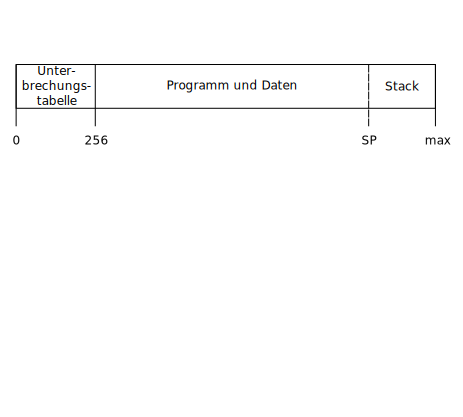
\includegraphics{./img/UMach-Speicherstruktur}
 \caption[Speicherstruktur]
         {Speicherstruktur zur Laufzeit. Die Begrenzungen zwischen den
          Segmenten werden durch konstante Zahlen oder Registerinhalte
          angegeben. Von diesen sind lediglich die Register \texttt{SP}
          und \texttt{HE} veränderbar, alle anderen sind, nach dem Laden des
          Programms in den Speicher, fest.}
 \label{fig:Speicherstruktur}
\end{figure}



\subsection{Interrupttabelle}
\index{Interrupttabelle}
\label{subsubsec:Interrupttabelle}

Die Interrupttabelle besteht aus einer Reihe von 32-Bit langen Sprungadressen
zum ausführbaren Code, bzw. zu sogenannten Interruptroutinen, oder auch \glqq
Interrupt Handlers\grqq, die in Ausnahmefällen ausgeführt werden sollen. Jedes
mal, wenn eine Ausnahmesituation auftritt (meistens eine Fehlersituation), wird
intern ein Interruptsignal erzeugt, das mit einer Kennnummer (Interruptnummer)
versehen ist. Die Interruptnummer wird zur Berechnung eines Index in dieser
Tabelle verwendet.


Die Interrupttabelle wird nicht von der Maschine gefüllt, sondern es ist
Aufgabe des Maschinenprogramms bei Bedarf entsprechende Einträge der
Interrupttabelle zu füllen und die zugehörige Funktionalität bereit zu stellen.
Ist eine Interrupadresse nicht gesetzt, d.h. ist der entsprechende
Tabelleneintrag Null, so reagiert die Maschine auf die Ausnahmesituation
indem sie hält. Für weitere Informationen bzgl. der Fehlerbehandlung siehe den
Abschnitt \ref{sec:Interrupts}, ab der Seite \pageref{sec:Interrupts}.

Die Interrupttabelle besteht aus 64 Einträgen, die 64 möglichen Interrupts
entsprechen. Jeder Eintrag beträgt wie ein Register 32 Bit, oder 4 Byte. Da es
64 Einträge gibt, ist die Interrupttabelle $64 \cdot 4 = 256$ Bytes groß. Die
Interrupttabelle fängt an der Adresse Null an. Siehe auch Abbildung
\ref{fig:Speicherstruktur} auf Seite \pageref{fig:Speicherstruktur}.

Die Berechnung der Adresse eines Interrupt-Handelers aus der Interruptnummer
erfolgt durch Multiplizieren mit 4 der Interruptnummer. Also für sine
Interruptnummer $n$ wird die Adresse $a$ wie folgt berechnet:
\[
    a = 4 \cdot n
\]
Als Beispiel, aus der Interruptnummer $n = 16$ wird die Adresse 
$a = 4 \cdot 16 = 64$ berechnet. An dieser Adresse wird die Adresse einer
Subroutine gesucht, die als Interrupt-Handler gestartet wird -- bzw. dort
gesprungen wird.

Tabelle \ref{tab:Interrupttabelle} auf Seite \pageref{tab:Interrupttabelle}
listet alle definierten Interruptnummern\index{Interruptnummer} und deren
Bedeutung auf.


\subsection{Programm und Daten}
\label{subsec:Prog-Daten}
\index{Programm}

Nach der $256$ Bytes ($64$ mal $4$) großen Interrupttabelle
folgt das eigentliche Programm, das von der Maschine ausgeführt werden soll.
Insbesondere ist dieses Programm dafür zuständig, die Interrupttabelle zu
füllen, falls (bestimmte) Interrupts behandelt werden sollen.


Das Programmsegment\index{Programmsegment} fängt an der Adresse $256$ an und ist
schreibgeschützt. Es enthält eine Kopie der ausführbaren Instruktionen aus
der Programmdatei.

Das Datensegment\index{Datensegment} folgt nach dem Programmsegment. Seine
Anfangsadresse wird im Register $DS$\index{DS@\texttt{DS}} gespeichert. Seine
Größe ist fest und wird durch die Anzahl der Datenbytes bestimmt. Dieses Segment
enthält eine Kopie der Daten, die in der Programmdatei eingebettet sind.
Das Datensegment ist nicht schreibgeschützt.

\subsection{Heap und Stack}
\label{subsec:Stack}
\index{Heap}
\index{Stack}

Nach dem Datensegment folgt das Heap-Segment.\index{Heap} Seine Anfangsadresse
wird im Register \texttt{HS}\index{HS@\texttt{HS}} gespeichert. Dieses Segment,
oder Speicherbereich, steht dem Programmierer frei. Das Ende des Heap-Bereichs
wird durch den Inhalt des Registers \texttt{HE}\index{HE@\texttt{HE}} markiert.
Der Heap belegt also alle Speicheradressen aus dem Interval $[\$HS, \$HE]$,
wobei $\$HS$ und $\$HE$ die Inhalte der Register \texttt{HS} und \texttt{HE}
bezeichnen.


Der Stack ist ein spezieller Bereich im Speicher. Dieser Bereich fängt am Ende
des Speichers mit der größten Adresse an und erstreckt sich bis zur derjenigen
Adresse, die im Register \texttt{SP}\index{SP@\texttt{SP}} gespeichert ist. Die
Stack-Größe ist damit dynamisch, denn das Register \texttt{SP} wird sowohl durch
die Instruktionen \opref{PUSH} und \opref{POP}, als auch direkt vom
Programmierer geändert.

Das Wachsen\index{Stack!Wachsen} des Stacks bedeutet, dass das Register
\texttt{SP} immer kleinere Werte annimmt. Das Schrumpfen\index{Stack!Schrumpfen}
des Stacks bedeutet, dass \texttt{SP} immer größere Werte annimmt.

Beim Hochfahren der Maschine, wird das Register \texttt{SP} auf die
maximal erreichbare Speicheradresse plus Eins gesetzt. Damit können keine Werte
gelesen werden, bevor Werte geschrieben wurden.



\subsection{Speicher Fehler}
\label{subsec:Speicherfehler}

Bei der Speicheraddressierung können während der Programmausführung
verschiedene Fehler auftreten.

\paragraph{Ungültige Speicheradresse}
Falls das Programm eine nicht-existierende Speicheraddresse anspricht, wird von
der Maschine der entsprechende Interrupt erzeugt. Folgende Fälle zählen dazu:
\begin{enumerate}
 \item Schereiben oder Lesen an Adresse kleiner Null.
 \item Schereiben oder Lesen an Adresse größer als die maximal erreichbare
       Adresse.
\end{enumerate}


\paragraph{Zugriffsverletzung}
\index{Zugriffsverletzung}

Eine Zugriffsverletzung (ähnlich einer \glqq segmentation fault\grqq, oder
\glqq segfault\grqq) \index{segfault} liegt vor, wenn Schreibrechte
eines Segments verletzt werden, oder wenn die Grenzen eines Segments
überschritten werden. Konkret sind die folgenden Fälle eine Zugriffsverletzung:
\begin{enumerate}
 \item Schreiben im Programmsegment.
 \item Register \texttt{HE} auf einer Adresse größer oder gleich der Adresse in
       \texttt{SP} setzen (Heap Überlauf\index{Heap!Überlauf}).
       \index{HE@\texttt{HE}}
 \item Register \texttt{SP} auf eine Adresse größer als die maximal erreichbare
       Adresse setzen (auch durch den \opref{POP} Befehl).
\end{enumerate}



\paragraph{Stack Überlauf}
\index{Stack!Überlauf}
Ein Stack Überlauf liegt vor, wenn der Stack Pointer (Register \texttt{SP})
\index{SP@\texttt{SP}} auf eine Speicheradresse kleiner gleich dem Wert des
Registers \texttt{HE} gesetzt wird. Mit anderen Worten, wenn der Stack das
Daten-, Programm- oder Heap-Segment überlappen würde.


\subsection{Speicheradressierung}
\index{Speicheradresse}

Um die Komplexität der UMach Maschine gering zu halten, kennt die vorliegende
Version lediglich absolute Adressen. Konzepte wie virtuelle Adressen,
Prozesse\index{Prozess} und getrennte Addressräume für Prozesse werden nicht
unterstützt. Wird versucht, den Inhalt einer Speicheradresse zu lesen oder zu
schreiben, so wird die angegebene Adresse nicht übersetzt oder modifiziert,
sondern direkt verwendet.

